% Asset ID: AS1TrigonometricRatiosTIKZ-004
% Source: P1-Chp9 pp.13-15
% Related section: Sine Rule
% Purpose: Sine rule opposite pairs
\documentclass[tikz,border=8pt]{standalone}
\usepackage{amsmath}
\usetikzlibrary{angles,quotes,calc,arrows.meta}
\begin{document}
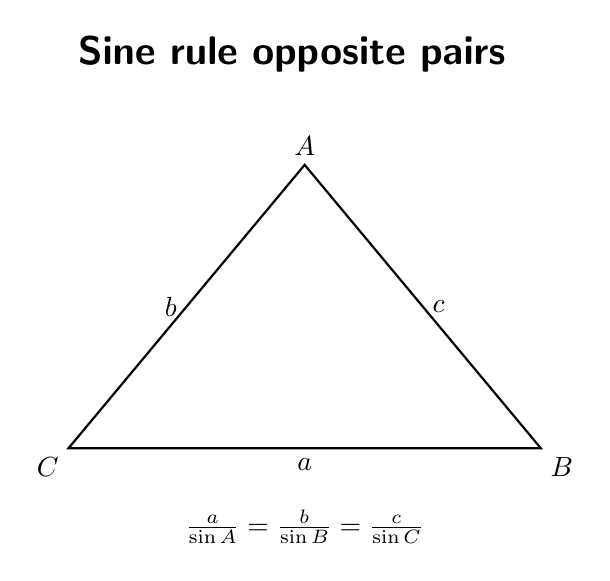
\begin{tikzpicture}[scale=1.0, every node/.style={font=\sffamily}]
\node[font=\sffamily\bfseries\Large, anchor=west] at (0,5) {Sine rule opposite pairs};
\coordinate (A) at (3,3.6);\coordinate (B) at (6,0);\coordinate (C) at (0,0);\draw[thick] (A)--(B)--(C)--cycle;\node[above] at (A) {$A$};\node[below right] at (B) {$B$};\node[below left] at (C) {$C$};\node[below] at ($(B)!0.5!(C)$) {$a$};\node[left] at ($(A)!0.5!(C)$) {$b$};\node[right] at ($(A)!0.5!(B)$) {$c$};\node at (3,-1) {$\frac{a}{\sin A}=\frac{b}{\sin B}=\frac{c}{\sin C}$};
\end{tikzpicture}
\end{document}
